\begin{marginfigure}
\begin{tikzpicture}
\node [name-dest] (box){%
    \begin{minipage}{0.80\textwidth}
    \begin{itemize}
    \item Sam Page
    \item James 'Tetley' Hooper
    \end{itemize}
    \end{minipage}
};
\node[fancytitle, right=10pt] at (box.north west) {Beetle Juice---Altantis};
\end{tikzpicture}
\end{marginfigure}

\section{A mysterious companion}

\subsection{20-7-13}

\paragraph{Tetley 5.30pm}
Smooth journey down with Sam. Good to be back for the 5th year that there’s been a camp at X-ray - like the other X-ray it’s hard to shut down! The camp looks as nice as ever... Off soon to push leads in Milky Way.

\paragraph{Sam}
Back down at X-ray. Lovely as ever, it’s strange how more comfortable I fell down here than I did on my first visit last year. The whole procedure of getting/leaving here is much less daunting than before and indeed we are soon off caving having drank tea and eaten smash. I’m looking forward to sleeping all the comf, currently residing behind me, later tonight.


\subsection{21-7-13}

\begin{marginfigure}
\checkoddpage \ifoddpage \forcerectofloat \else \forceversofloat \fi
\centering
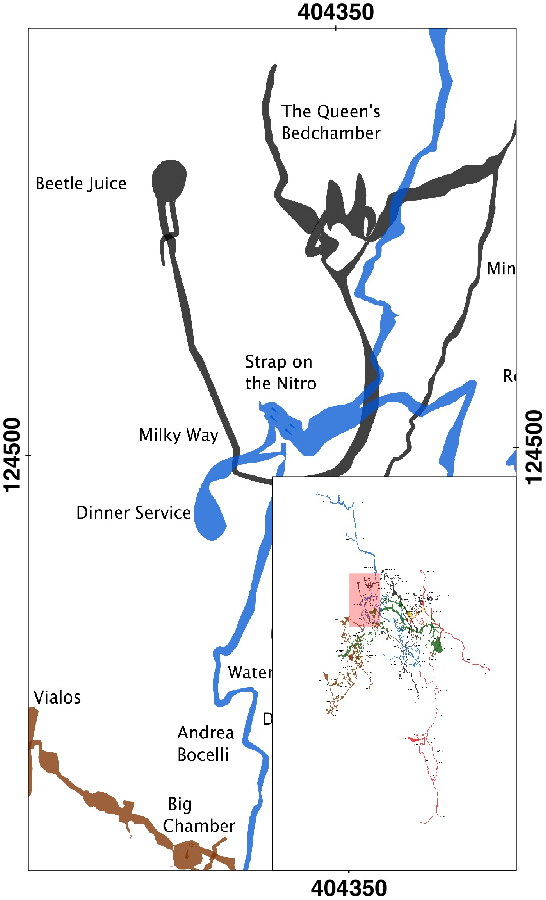
\includegraphics[width=\textwidth]{images/2013/tetley-sam-2013/beetlejuice_inset.pdf}
\caption{Beetle juice and the Milky Way area (black) lie close to the connection between \emph{Vrtnarija} and \emph{Sistem Migovec} --- Slovenian National Grid EPSG 3794 }
\label{small inset}
\end{marginfigure}

\paragraph{Sam 4.20am}
Eating and drinking back at camp at this ungodly hour. I have no idea which train, if any, we are currently riding...Arrived back at camp close to an hour ago after pushing the pitch and consequent rift at the end of Milky Way, which is BEETLE JUICE. My last pushing trip last year had been to Milk Way and myself and Clare had poked our heads over a promising looking pitch under a load of boulders, which has then been rigged and descended with a rift at the bottom which had been left last year. Tetley slightly rerigged the pitch (basically backing up and avoiding the water). At the bottom there was indeed a rift leading off. This seemed fairly promising and soon came another pitch above which Tetley bolted and rigged a y-hang at the bottom of which...Beetle Juice died :( There was a ‘vertical fault crack’ (thanks Tetley) on either side of the pitch bottom bringing our pushing trip to an end and probably making us both the first and last people to ever set foot there. Still, added metres shouldn't be sniffed at and according to Tetley Beetle Juice might necessitate some slight altering of the survey. Fatigue started to set in towards the end of the night wore on and my patience was definitely pushed whilst descending Apollo, truly the worst thing ever. Plan now is to sleep until who knows when and then go push elsewhere (Atlantis?) later on. We’re not expecting to share camp with anyone else over the course of our stay which is probably a good thing considering out messed up timetable.
Thanks Tetley for a great day (and night...). 



\begin{quote}Though your protestation of me doing the breaking may not be borne by my aching body. \end{quote} 
[Ed - No idea]


\paragraph{Tetley 5.00am}
A great day’s caving - my first without glasses! Longer than I bargained for... more after sleep. Listening to one of Clare’s great playlists, full of tea, noodles and smash. Whiskey now and glorious sleep (55 metres surveyed today).

\paragraph{Sam 2.55pm}
Just woke up after a great and long nights sleep. Time truly has no meaning down here...


\paragraph{Tetley 4.00pm}
It’s amazing that we;re now living in a 25+km long system - the result of 39 years of pushing by JSPDT and 19 years by $IC^3$ The Apollo climb was an awesome pitch, I was truly impressed - it’s also now a truly horrible pitch, it should be rerigged if it becomes a ‘trade route’. Writing of connections, a ‘super action’ is going on now to connect Monatip to the system, hopefully this one will prove easier than the M2-Captain K effort that after years of toil, never (to date!) occurred!


\paragraph{Tetley 4.35pm}
Just listened to ‘Come on Baby Light my Fire’ - while burning toilet paper in the new ‘toilet paper burner’ - a great addition to our facilities!
P.S. Sadly fairy lights not working :( but I like the coat hangers :-)!

\paragraph{Tetley 6.00pm}
Morning rituals, ablution etc. completed (including two episodes of Blackadder naturally). Getting changed now to head off to Atlantis.


\paragraph{Sam 6.02pm}
Oh man, getting changed will be cold!

\subsection{22-7-13}

\paragraph{Sam 8.40am}
Just back from our trip and I am ever so slightly broken...
More Importantly, WE ARE NOT ALONE! Me and Tetley saw a fucking animal at Hawaii. It was some sort of mix between a rat and a squirrel, black with a long fluffy black tail. Something like this. 
[Crude drawing of squirrel rat goes here]
After I sat down I turned my head an it was just there. My first reaction was to ask Tetley “What is THAT?”; his first reaction was to scream as it moved and ran away. I probably watched it for around ten seconds before it disappeared. Where did it come from to end up at -800m!?! Does this mean there is an entrance somewhere around there. How could it get to where we were; it looked like it was moving well yet was spooked by us. We too were spooked by it. Surely it and more of it’s kind don’t live down here with us? First action when back on the surface is to find out if such a creature exists.
P.S. Creature Theories
\begin{itemize}
\item 1. Saber brought it down in a cage and released it
\item 2. It came from outside
\item 3. Tetley and Sam had a mad hallucinogenic trip
\item 4. An alien invasion of Sys Mig
\item 5. A creature to revolutionise all known biology - where does it get its light/food from???
\item 6. Magic
\end{itemize}
According to Tetley Hawaii is nowhere near the surface. WHAT THE ACTUAL FUCK DID WE SEE!!!

\begin{figure}[t!]
	\checkoddpage \ifoddpage \forcerectofloat \else \forceversofloat \fi
	\centering
	\frame{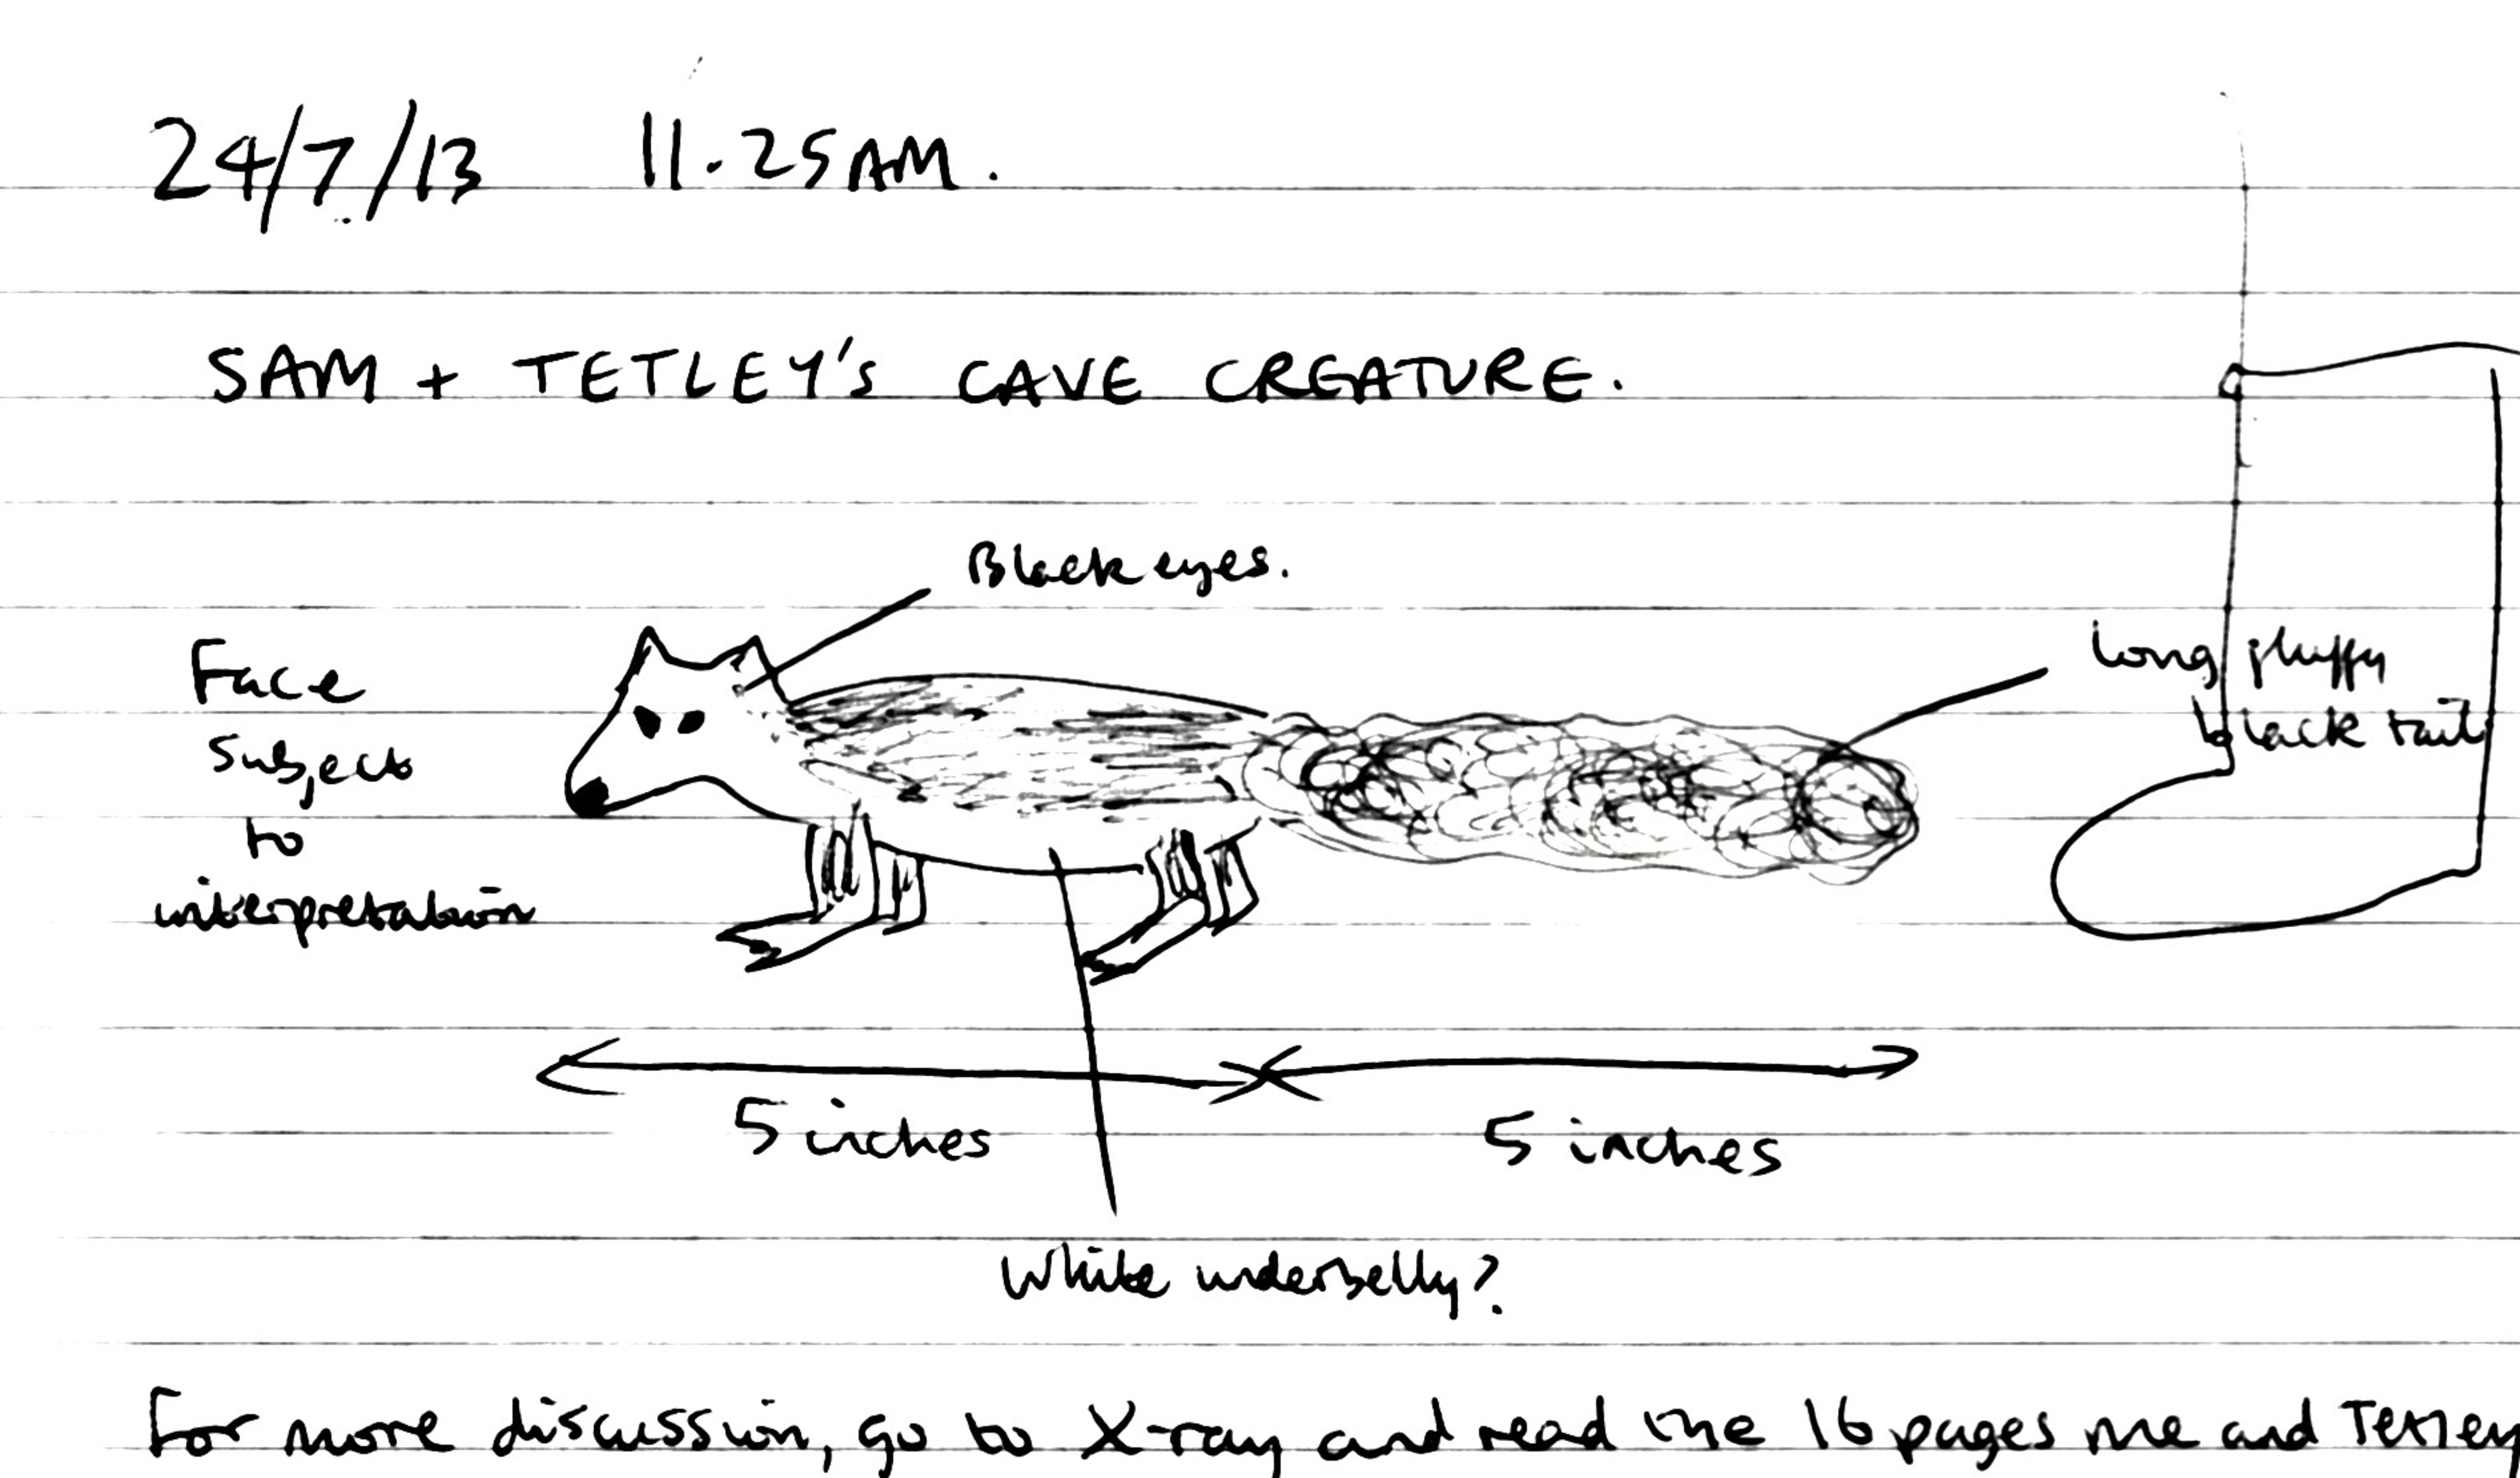
\includegraphics[width=\textwidth]{images/2013/tetley-sam-2013/creature.pdf}}
	\caption{The creature spotted by Sam and Tetley, drawn in the 2013 scanned logbook --- scanned, from Sam Page}
	\label{the creature}
\end{figure}

\paragraph{Tetley 9.50am}
Firstly before I forget.
HAPPY BIRTHDAY PETE
from Camp X-Ray !!!!
Earlier today I said Mig gives up its secrets slowly but at around 3.40am I saw the creature at Hawaii previously described. I have NO RATIONAL EXPLANATION... IT must have come from outside...but how??????
Hawaii is about 120m east and 750m below the entrance to M16. Now sleep, glorious sleep....

\begin{marginfigure}
\checkoddpage \ifoddpage \forcerectofloat \else \forceversofloat \fi
\centering
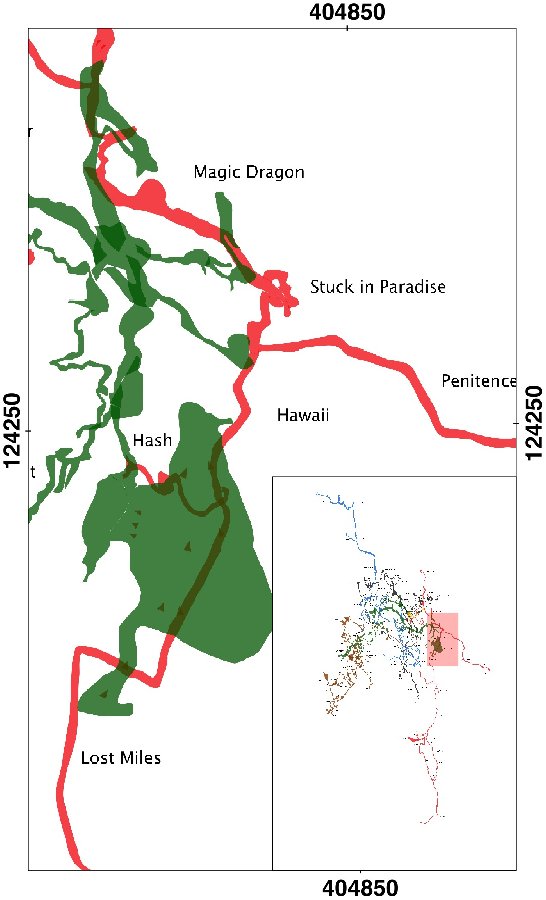
\includegraphics[width=\textwidth]{images/2013/tetley-sam-2013/hawaii_inset.pdf}
\caption{\emph{Hawaii} lies at the junction between the two horizontal galleries Penitence and Lost Miles which head east and south  respectively --- Slovenian National Grid EPSG 3794 }
\label{small inset}
\end{marginfigure}

\paragraph{Tetley 7.30pm}

So our trip yesterday... a smooth journey down to Hawaii. Stuck in Paradise is much much better than when I first went down but still somewhat muddy and loose. Sam’s first trip to this part of the cave. We had vitaminski tea and hot fish sandwiches. Went to push HASH, added 25m (Sam described this earlier). The leas isn’t great but it is still draughting and going. We then went to see the nice stal at Atlantis, very pretty! Back to Hawaii for tea...Sam was ahead of me and as I neared Hawaii said, with I detected a slight anxious tone in his voice, “Tetley, tetley look at this”. I was thinking maybe he was watching a spider or something...I approached and there to my surprise (to put it mildly) was a rat type creature. It moved! I screamed!. What! Why? How? We had some ginger cake (leaving some for the creature), also had some vitaminski tea. Dumbfounded we headed back to camp/ I had the previously mentions explosive shit on ledge after Kamikaze breakthrough point. Also of note, I bought, for £40 or so, a non-Petzl chest jammer a month ago. It’s shit, the rope doesn't pull though and it’s very hard to open. This is the first and last trip that I will use it. Hope journey out isn’t too frustrating with this crap piece of equipment. Caveat Emptor indeed! Talking of Petzl, as a boy I read his tales of cave exploration, also the stories of Dent de Crolles, PSM, Gouffre Berger etc. Looking now at the survey of our 25km system (hopefully now 30km+ if Primadona/Monatip has now connected in) it really is amazing, truly amazing, that we’ve a tale and a cave of similar magnitude!
I’m feeling sleepy again so I’ll spare you my musing on love/relationships...






\paragraph{Tetley 11.58pm}
P.S. it’s still just Sam and me here and we’ve still got 36 hours to our callout...I think more dossing/sleeping is on the cards!


\subsection{23-7-13}


\paragraph{Tetley 4.40am}
After 17 hours with only the sound of the stream and Sam’s breathing I felt the need for some tea! Decided to listen to Rum Doodle...the episodes on the player are not in the right order - the correct order is 4,1,2,5,3. We’re low on sugar and have no champagne - lassitude sickness perhaps.

\begin{figure*}[t!]
\checkoddpage \ifoddpage \forcerectofloat \else \forceversofloat \fi
\centering
\frame{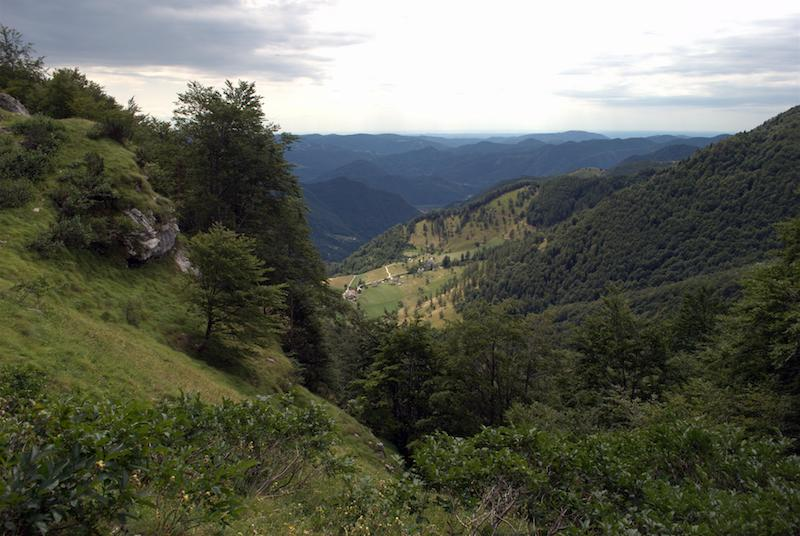
\includegraphics[width=\textwidth]{images/2013/tetley-sam-2013/path-below-kal.jpg}}
\caption{\emph{Hawaii} is at least 1km away from the outer surface in the horizontal plane - our current hypothesis is that the small mammal is a dormouse who entered somewhere below the Sheperd's Hut and made its way along the horizontal passages leading to Hawaii eg. \emph{Atlantis}--- scanned, from Sam Page }
\label{the creature}
\end{figure*}

\paragraph{Sam 5.20am}
Been at x-ray for an awfully -wrong word- brilliantly long time now. I don't expect I would have been able to sleep for 17 hours on the surface. 3 days of just Tetley and I (plus our mysterious creature still preoccupying our thoughts) - where have all the cavers gone? Presumably the connection with Monatip/B12/the Bivvy have proven too distracting. Plan is to head out at some point today, as long as we are out for sunset. Before that, food, more sleep, Rum Doodle, Blackadder....good times.


\paragraph{Sam 5.40am}
Tet’s gone all philosophical...


\paragraph{Tetley 6.10am}
6 billion people on the planet and no-one can have had a weekend like the one Sam and I had! Now eating cheesy, soupy, fishy, smash (classic! with - and highly recommended - fresh onion. More Rum Doodle, Black Adder, sleep now...

\begin{figure}[t!]
\checkoddpage \ifoddpage \forcerectofloat \else \forceversofloat \fi
\centering
\frame{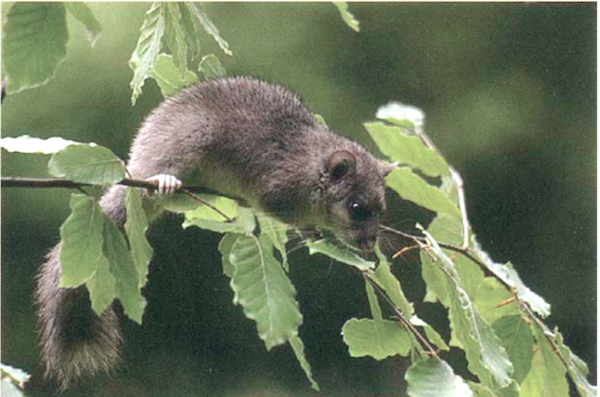
\includegraphics[width=\textwidth]{images/2013/tetley-sam-2013/dormouse.png}}
\caption{Adult \emph{Glis Glis} from Mt. Kocevski Rog, Slovenia --- photo courtesy of A Kry\v{s}tufek  }
\label{the creature}
\end{figure}

\begin{figure*}[b!]
\begin{tikzpicture}
\node [name-dest] (box){%
    \begin{minipage}{0.95\textwidth}
    \begin{multicols}{2}
    \paragraph{General characters of the dormouse}  The edible dormouse \emph{Glis Glis} is the largest of its genus and has the appearance of a squirrel. Both sexes are roughly the same size with a body of length averaging 15.3cm, and tail measuring 12.5cm \citep{kryvstufek2001compartmentalisation}. Its pelage consist of a soft underfur, mixed with coarser, longer guard hairs along the back. The fur ranges from grey-brown to smoke-grey and is darkest along the spine. The underparts are white to pale buff, and the transition is clearly defined. The tail has the same colour as the back, albeit darker. 
    
    \paragraph{distribution} \emph{Glis Glis} is widespread in the deciduous western, central and southeastern Europe except near the Atlantic and North sea coasts.  It is found from sea level to the upper margins of deciduous and mixed forests, at elevations of up to 2000m in the Pyrenees \citep{spitzenberger2001saugetierfauna}. The edible dormouse, very widespread in Slovenia \citep{kryvstufek1991sesalci} is a nocturnal arboreal rodent which uses tree hollows, as well as burrows to breed. Their occurrence in caves has been known about for centuries \citep{von1994slava}, as Slovene hunters caught the fat dormice outside \emph{pol\v{s}ine}, very small entrances (5 -10cm diameter) to larger cave systems, where the rodents are found to nest and hibernate \citep{scaravelli1995myoxus}.
      
    \paragraph{occurrence in caves} Dormice commonly occur in caves of the Slovene Dinaric karst, a mountainous area covered with a mixture of beech (\emph{Fagus Sylvatica}) and fir (\emph{Abieti-fagetum dinaricum}) forests \citep{polak1997}.

 \end{multicols}{2}
    \end{minipage}

};
\node[fancytitle, right=10pt] at (box.north west) {More about the edible dormouse \emph{Glis Glis}};
\end{tikzpicture}
\end{figure*}


\paragraph{Tetley 10.30am}
After some more sleep (basically 24 hours in bed with food, tea, cigarette, shitting breaks) we’ve stirred again. Used an old peanut choco and an old Double Decker to make a tasty hot choc in the small pan. I’ve started to think of the surface, the sun, sitting round the bivvy fire etc. We’ve decided against a 3rd days pushing and will certainly be out before sunset. I think the Imodium has worked (touch rock!).
Yet again we’ve discussed the numerous scientific, philosophical and psychological questions posed by our sighting of the creature. 
\begin{itemize}
\item What was it?
\item How did it get there?
\item Did we really see it? (Yes, we both agree)
\item Can the scientifically impossible actually occur? (I don’t want to believe this)
\item Our mutual reaction to the creature and it’s implications.
\item How will the other cavers react?
\end{itemize}


\paragraph{Tetley 11.35am}
The time has come to go...
Final brew on the stove, will soon change into furry. Thanks for the great company Sam, an unforgettable camp at X-Ray, only 80m surveyed but good caving, good fun, good dossing and a probably once in a lifetime/unique encounter.
Looking forward to a good sesh round the fire, bowels ok. Hope chest jammer not too irksome.
Good caving and pushing to the teams that follow - and I hope you find reading the logbook a good read!


\paragraph{Sam}
Starting the inevitable crawl towards the surface...it’ll be good to be back on the top after a long - but brilliant- time underground. Cheers Tetley for great caving/dossing. I apologise for my grouchy, grumpy side that seems to come out towards the end of every pushing trip...but camp soon puts things right. Towards the orb!


\paragraph{Tetley 12.55pm}
Out now for sun, sunset etc. Two beers await on the surface! Thanks again Sam.


\paragraph{Sam 1.00pm}
‘Til next time, X-ray!


